\chapter{Declarative Geometry Constraint Solver}
\label{chap:declarative}

\section{Overview}

The third module is a declarative geometry constraint solver. Given a
user-specified topology of a diagram and various constraints on
segments and angles, this module attempts to solve the specification
by instantiating a figure that satisfies the constraints.

The solver is implemented using propagators, uses new types of partial
information about point regions and direction intervals, and focuses
on emulating the mental process of wiggling constrained figures in the
mind's eye. The physical nature of this process is captured by forming
analogies between geometry diagrams and mechanical linkages of bars
and joints.

After providing a brief overview of the mechanical analogies and quick
background on the propagator system, I examine an example of the
system solving a set of constraints for an under-constrained
rectangle. Then, I describe the module implementation, starting with
the new partial information representations and linkage constraints
before explaining how mechanisms are assembled and solved. Finally,
some limitations and extensions are discussed.

%% Outline
%% - Mechanical Analogies
%% - Propagator System
%% - Partial Information Structures
%% - Linkages
%% - Building a Mechanism
%% - Solving a Mechanism
%% - Discussion

\subsection{Mechanical Analogies}

Mechanical analogies are often applied to mathematical problems to
yield alternate, sometimes more-intuitive solutions. Several texts
such as [??], [??], and [??] study this and provide examples.

In this system, mechanical analogies are used to represent the physics
simulation going on as one mentally manipulates a diagram ``in the
mind's eye''. Often, given a diagram with constraints, one can imagine
assembling a physical example of the figure out of bars and joints in
one's head.  Some bars can be sliding to make their lengths adjustable
whereas others are constrained to be of equal length as one another.
As a person moves and wiggles these pieces to assemble satisfying
mechanisms, they can examine whether the resulting mechanisms retain
properties across instances and generalize such invariants into
theorems.

This module simulates this process by assembling mechanisms of bars
and joints, and using a propagator system to simulate incrementally
selecting where bars and joints are positioned while maintaining local
physical constraints.

\subsection{Propagator System}

The declarative geometry solver is built upon an existing propagator
system created by Alexey Radul under the advisement of Gerald Jay
Sussman \cite{gjs-propagator}. The propagator system allows a user to
create cells and connect them with propagator constraints. As content
is added to cells, their neighbors are notified and updated with
computations performed on the new information. Often, cells maintain a
representation of partial information about their content and merge
new information from several sources.

This module uses Radul's propagation system to handle the underlying
propagation of data, but implements constraints, partial information
types, specification protocols, and input formats particular to geometric
figures.

\section{Example of Solving Geometric Constraints}
\label{sec:example-solving}

I begin by fully explaining an example. The geometry problem of
inadequately constrained rectangles was introduced in the first
example of Chapter~\ref{chap:motivation} on page
\pageref{example-1}. The second proposed set of constraints in that
problem was expressed as a mechanism in Example~\ref{is-rect-2} in the
demonstration (page \pageref{is-rect-2}), and is repeated here in
Example~\ref{is-rect-specs}. Example~\ref{is-rect-solved} shows the
module's print messages as it solves the mechanism.

The illustrations in Explanation~\ref{illustration} and accompanying text
on the following pages explain how propagation is used to solve this
mechanism.

\begin{code-example}
[label=is-rect-specs]
{Rectangle Constraints Example}
(define (is-this-a-rectangle-2)
  (m:mechanism
   (m:establish-polygon-topology 'a 'b 'c 'd)
   (m:c-length-equal (m:bar 'a 'd) (m:bar 'b 'c))
   (m:c-right-angle (m:joint 'd))
   (m:c-angle-equal (m:joint 'a) (m:joint 'c))))
\end{code-example}

\begin{img-example}
[label=is-rect-solved]
{Solved Constraints}{images/rect-demo-2.png}
=> (m:run-mechanism (is-this-a-rectangle-2))

(specifying-bar m:bar:d:a .6742252545577186)
(initializing-direction m:bar:d:a-dir (direction 4.382829365403101))
(initializing-point m:bar:d:a-p1 (0 0))
(specifying-joint m:joint:c:b:a 2.65583669872538)
\end{img-example}

Solving a mechanism involves repeatedly selecting positions, lengths,
angles, and directions that are not fully specified and selecting
values within the domain of that element's current partial
information. As values are specified, the wiring of the propagator
model propagates further partial information to other values.

\refstepcounter{tcb@cnt@code-example}\label{illustration}
\begin{figure}[h]
\captionsetup{labelformat=empty}
\caption{{\bf Propagation Explanation
    \arabic{chapter}.\arabic{tcb@cnt@code-example}:} This series of
  illustrations depicts the propagation steps that occur to enable the
  system to solve the underconstrained rectangle from
  Example~\ref{is-rect-specs}.
}
\centering
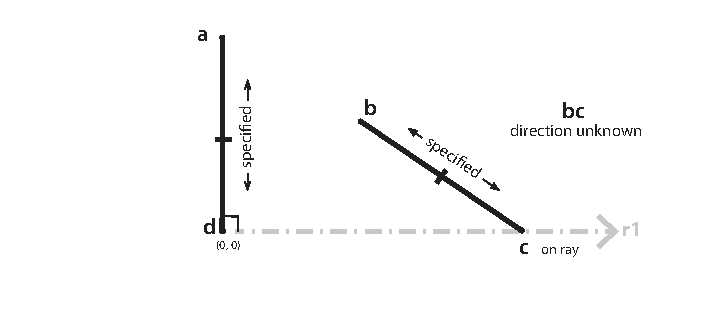
\includegraphics[width=.95\textwidth]{diagrams/is-rect-explained-boards-1.eps}
\caption{{\bf Step 1:} The first value the module specifies is the
  length of bar \texttt{ad}. In doing so, it also initializes the
  bar's endpoint and direction to anchor it on the canvas. Because
  joint \texttt{d} is constrained to be a right angle, the system knows
  the direction but not length of bar \texttt{dc}. It propagates the
  partial information that point \texttt{c} is on the ray $r1$ extending
  out from \texttt{d} to the cell within point
  \texttt{c}. Furthermore, since bars \texttt{ad} and \texttt{bc} are
  constrained to have equal length, at this point, bar \texttt{bc} also knows
  its length but not direction. Next, the system specifies joint angle \texttt{b}:}
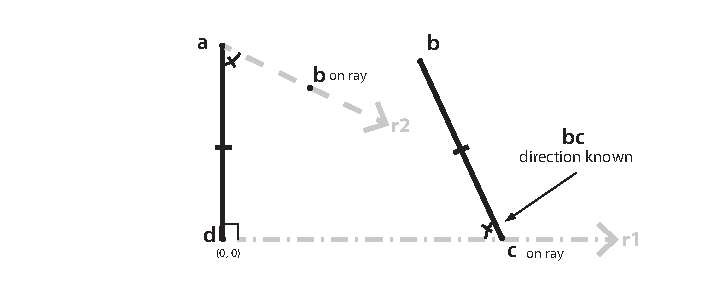
\includegraphics[width=.95\textwidth]{diagrams/is-rect-explained-boards-2.eps}
\caption{{\bf Step 2:} Once the angle measure of \texttt{b} is
  specified, constraints using the sum of angles in the specified
  polygon and a ``slice'' constraint on the pair of constrained angles
  will set the angle measures of joints \texttt{a} and \texttt{c} to
  be half of the remaining total:
  $\text{\texttt{a,c}}\protect\leftarrow\frac{2\protect\pi -
    \text{\texttt{b}} - \text{\texttt{d}}}{2}$. With these angles
  specified, point \texttt{b} is informed that it is on the ray $r2$
  and bar \texttt{bc} now knows both its length and direction.}
\vspace{-10em}
\end{figure}

\newpage
\begin{figure}[h]
\captionsetup{labelformat=empty}
\caption{{\bf Propagation Explanation
    \arabic{chapter}.\arabic{tcb@cnt@code-example} continued:} This series of
  illustrations depicts the propagation steps that occur to enable the
  system to solve the underconstrained rectangle solved in
  Example~\ref{is-rect-specs}.}
\centering
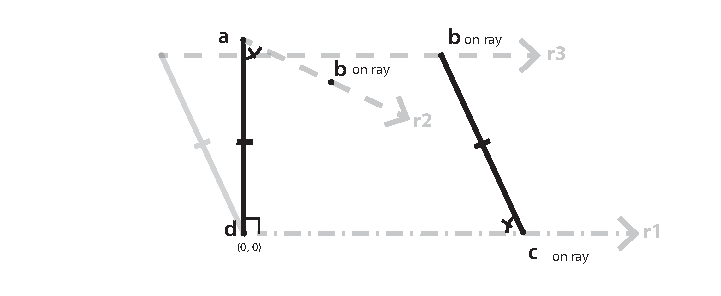
\includegraphics[width=.95\textwidth]{diagrams/is-rect-explained-boards-3.eps}
\caption{{\bf Step 3:} Since now both the length and direction of bar
  \texttt{bc} are known and point \texttt{c} is known to be on ray
  $r1$, the propagation constraints can translate this ray by the
  length and direction of \texttt{bc} and provide the information that
  point \texttt{b} must therefore also be on ray $r3$. This emulates
  the physical process of sliding bar \texttt{bc} along ray $r1$.}
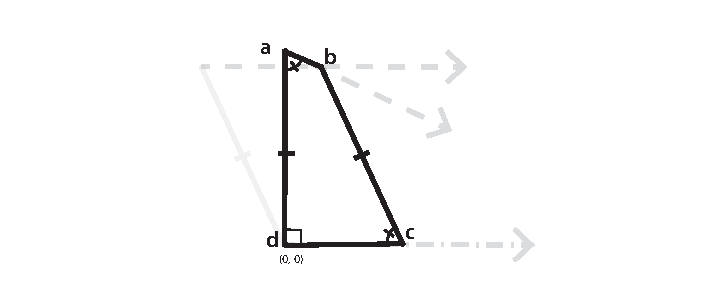
\includegraphics[width=.95\textwidth]{diagrams/is-rect-explained-boards-4.eps}
\caption{{\bf Step 4:} The information about point \texttt{b} being on
  rays $r2$ and $r3$ is merged via ray intersection to fully determine
  the location of \texttt{b}. Then, once point \texttt{b} is
  specified, since the length and direction of bar \texttt{bc} is
  known, propagation sets the value and location of point \texttt{c},
  yielding a fully-specified solution.}
\vspace{-1.5em}
\end{figure}
Similar steps allow propagation to solve specifications for many
figures including isoceles triangles, parallelograms, and
quadrilaterals from their diagonals. Several of these are shown in
Section \ref{demo:sec:declarative}. In cases when bars have their
length and one endpoint specified first, the propagators specify that
the other endpoint is on an arc of a circle. The next sections
describe the implementation of these partial information structures
before explaining linkages and how mechanisms are built and solved.

\newpage
\section{Partial Information Structures}

Radul's propagation system typically used numeric intervals for
partial information. The declarative constraint solver uses standard
some numeric intervals, but also

\subsection{Regions}

Propagating partial information across bars and joints yields a new
region system: Regions include point sets of one or more possible
points, an entire ray, or an entire arc. These rays and arcs are
from an anchored bar with only one of direction or length specified,
for instance.

\begin{code-listing}
[label=regions]
{Region Structures}
(define-record-type <m:point-set>
  (%m:make-point-set points)
  m:point-set? ...)

(define-record-type <m:arc>
  (m:make-arc center-point radius dir-interval)
  m:arc? ...)

(define-record-type <m:ray>
  (%m:make-ray endpoint direction)
  m:ray? ...)

(define-record-type <m:region-contradiction>
  (m:make-region-contradiction error-regions)
  m:region-contradiction? ...)
\end{code-listing}

\subsection{Direction Intervals}

Ranges of intervals. Full circle + invalid intervals. Adding and
subtracting intervals of direction and thetas gets complicated at times.

Challenges with intersection, multiple segments. Eventually just
return nothing is okay.

\section{Linkages and Basic Constraints}

The solver uses bar and joint linkages.

Bars have endpoints, directions and length. Joints have a vertex point
and two directions. Currently, most joints are directioned and have
max value of 180 degrees.

\begin{code-listing}
[label=point-region]
{Points and Regions}
(define (m:make-point)
  (let-cells (x y region)
    (p:m:x-y->region x y region)
    (p:m:region->x region x)
    (p:m:region->y region y)
    (%m:make-point x y region)))

(define (m:x-y->region x y)
  (m:make-singular-point-set (make-point x y)))
(propagatify m:x-y->region)

(define (m:region->x region)
  (if (m:singular-point-set? region)
      (point-x (m:singular-point-set-point region))
      nothing))
(propagatify m:region->x)
(propagatify m:region->y)
\end{code-listing}

\begin{code-listing}
[label=bar-struct]
{Vectors}
(define (m:make-vec)
  (let-cells (dx dy length direction)
    (p:make-direction (e:atan2 dy dx) direction)
    (p:sqrt (e:+ (e:square dx)
                 (e:square dy))
            length)
    (p:* length (e:direction-cos direction) dx)
    (p:* length (e:direction-sin direction) dy)
    (%m:make-vec dx dy length direction)))
\end{code-listing}

\begin{code-listing}
[label=bar-struct]
{Basic Bar Structure}
(define (m:make-bar bar-id)
  (let ((p1 (m:make-point))
        (p2 (m:make-point))
        (v (m:make-vec)))
    (c:+ (m:point-x p1) (m:vec-dx v)
         (m:point-x p2))
    (c:+ (m:point-y p1) (m:vec-dy v)
         (m:point-y p2))
    (let ((bar (%m:make-bar p1 p2 v)))
      (m:p1->p2-bar-propagator p1 p2 bar)
      (m:p2->p1-bar-propagator p2 p1 bar)
      bar)))
\end{code-listing}

\begin{code-listing}
[label=bar-propagator]
{Bar Propagator}
(define (m:p1->p2-bar-propagator p1 p2 bar)
  (let ((p1x (m:point-x p1))
        (p1y (m:point-y p1))
        (p1r (m:point-region p1))
        (p2r (m:point-region p2))
        (length (m:bar-length bar))
        (dir (m:bar-direction bar)))
    (p:m:x-y-direction->region p1x p1y dir p2r)
    (p:m:x-y-length-di->region p1x p1y length dir p2r)
    (p:m:region-length-direction->region p1r length dir p2r)))

(define (m:x-y-length-di->region px py length dir-interval)
  (if (direction-interval? dir-interval)
      (let ((vertex (make-point px py)))
        (m:make-arc vertex length dir-interval))
      nothing))
(propagatify m:x-y-length-di->region)
\end{code-listing}

\subsection{Joint Constraints}
\begin{code-listing}
{Joint Constraints}
(define (m:make-joint)
  (let ((vertex (m:make-point)))
    (let-cells (dir-1 dir-2 theta)
      (p:m:add-to-direction dir-1 theta dir-2)
      (p:m:add-to-direction dir-2 (e:negate theta) dir-1)
      (p:m:subtract-directions dir-2 dir-1 theta)
      (m:instantiate theta (make-interval 0 *max-joint-swing*) 'theta)
      (%m:make-joint vertex dir-1 dir-2 theta))))
\end{code-listing}

\section{User-specified Constraints}

\begin{code-listing}{User Constraints}
(define-record-type <m:constraint>
  (m:make-constraint type args constraint-procedure)
  m:constraint?
  (type m:constraint-type)
  (args m:constraint-args)
  (constraint-procedure m:constraint-procedure))

(define (m:c-length-equal bar-id-1 bar-id-2)
  (m:make-constraint
   'm:c-length-equal
   (list bar-id-1 bar-id-2)
   (lambda (m)
     (let ((bar-1 (m:lookup m bar-id-1))
           (bar-2 (m:lookup m bar-id-2)))
       (c:id (m:bar-length bar-1)
             (m:bar-length bar-2))))))
\end{code-listing}

Angle sum of polygon, or scan through polygon and ensure that the
angles don't not match. Example is equilateral triangle, for
instance... Could also observe always ``60 degrees'' as an interesting
fact and put that in as a constraint. They're alebgraically quite
similar, but my propagators currently don't perform symbolic algebra.

\subsection{Slices}

\begin{code-listing}
[label=sum-slice]
{Sum Slice}
(define (m:equal-values-in-sum equal-cells all-cells total-sum)
  (let ((other-values (set-difference all-cells equal-cells eq?)))
    (c:id (car equal-cells)
          (ce:/ (ce:- total-sum (ce:multi+ other-values))
                (length equal-cells)))))

(define (m:sum-slice elements cell-transformer equality-predicate total-sum)
  (let* ((equivalence-classes
          (partition-into-equivalence-classes elements equality-predicate))
         (nonsingular-classes (filter nonsingular? equivalence-classes))
         (all-cells (map cell-transformer elements)))
    (cons (c:id total-sum (ce:multi+ all-cells))
          (map (lambda (equiv-class)
                 (m:equal-values-in-sum
                  (map cell-transformer equiv-class) all-cells total-sum))
               equivalence-classes))))
\end{code-listing}

\begin{code-listing}
[label=poly-sum-slice]
{Polygon Sum Slice}
(define (m:polygon-sum-slice all-joint-ids)
  (m:make-slice
   (m:make-constraint 'm:joint-sum all-joint-ids
    (lambda (m)
      (let ((all-joints (m:multi-lookup m all-joint-ids))
            (total-sum (n-gon-angle-sum (length all-joint-ids))))
        (m:joints-constrained-in-sum all-joints total-sum))))))

(define (m:joints-constrained-in-sum all-joints total-sum)
  (m:sum-slice all-joints m:joint-theta
   m:joints-constrained-equal-to-one-another? total-sum))
\end{code-listing}

\section{Building Mechanisms}

The Mechanism in our declarative system is analogous to Figure,
grouping elements. Also computes various caching and lookup tables to
more easily access elements.

\begin{code-listing}
[label=mechanism-struct]
{Mechanism Structure}
(define-record-type <m:mechanism>
    (%m:make-mechanism bars joints constraints slices
                       bar-table joint-table joint-by-vertex-table)
    m:mechanism? ...)

(define (m:mechanism . args)
  (let ((elements (flatten args)))
    (let ((bars (m:dedupe-bars (filter m:bar? elements)))
          (joints (filter m:joint? elements))
          (constraints (filter m:constraint? elements))
          (slices (filter m:slice? elements)))
      (m:make-mechanism bars joints constraints slices))))
\end{code-listing}

\begin{code-listing}
[label=est-topo]
{Establishing Topology}
(define (m:establish-polygon-topology . point-names)
  (if (< (length point-names) 3)
      (error "Min polygon size: 3"))
  (let ((extended-point-names
         (append point-names (list (car point-names) (cadr point-names)))))
    (let ((bars (map (lambda (p1-name p2-name)
                       (m:make-named-bar p1-name p2-name))
                     point-names
                     (cdr extended-point-names)))
          (joints (map (lambda (p1-name vertex-name p2-name)
                         (m:make-named-joint p1-name vertex-name p2-name))
                       (cddr extended-point-names)
                       (cdr extended-point-names)
                       point-names)))
      (append bars joints
              (list (m:polygon-sum-slice (map m:joint-name joints)))))))
\end{code-listing}

\begin{code-listing}
{Building Mechanisms}
(define (m:build-mechanism m)
  (m:identify-vertices m)
  (m:assemble-linkages (m:mechanism-bars m)
                       (m:mechanism-joints m))
  (m:apply-mechanism-constraints m)
  (m:apply-slices m))
\end{code-listing}

\begin{code-listing}
[label=identifying-points]
{Identifying points}
(define (m:identify-into-arm-1 joint bar)
  (m:set-joint-arm-1 joint bar)
  (m:identify-points (m:joint-vertex joint)
                     (m:bar-p2 bar))
  (c:id (ce:reverse-direction (m:joint-dir-1 joint))
        (m:bar-direction bar)))

(define (m:identify-points p1 p2)
  (for-each (lambda (getter)
              (c:id (getter p1)
                    (getter p2)))
            (list m:point-x m:point-y m:point-region)))
\end{code-listing}

\section{Solving Mechanisms}

\begin{code-listing}
[label=solve-mechanism]
{Solving Mechanisms}
(define (m:solve-mechanism m)
  (m:initialize-solve)
  (let lp ()
    (run)
    (cond ((m:mechanism-contradictory? m)
           (m:draw-mechanism m c)
           #f)
          ((not (m:mechanism-fully-specified? m))
           (if (m:specify-something m)
               (lp)
               (error "Couldn't find anything to specify.")))
          (else 'mechanism-built))))
\end{code-listing}

\begin{code-listing}
[label=specify-something]
{Specifying and Instantiating Values}
(define (m:specify-something m)
  (or
   (m:specify-bar-if m m:constrained?)
   (m:specify-joint-if m m:constrained?)
   (m:specify-joint-if m m:joint-anchored-and-arm-lengths-specified?)
   (m:initialize-bar-if m m:bar-length-specified?)
   ...)

(define (m:instantiate cell value premise)
  (add-content cell
    (make-tms (contingent value (list premise)))))
\end{code-listing}


Given a wired diagram, process is repeatedly specifying values for elements


\subsection{Interfacing with existing diagrams}

Converts between figures and symbolic relationships.

\begin{code-listing}
[label=to-figure]
{Converting to Figure}
(define (m:mechanism->figure m)
  (let ((points (map m:joint->figure-point (m:mechanism-joints m)))
        (segments (map m:bar->figure-segment (m:mechanism-bars m)))
        (angles (map m:joint->figure-angle (m:mechanism-joints m))))
    (apply figure (filter identity (append points segments angles)))))
\end{code-listing}

\section{Discussion and Extensions}

Future efforts involve an improved backtrack-search mechanism if
constraints fail, and a system of initializing the diagram with
content from an existing figure, kicking out and wiggling arbitrary
premises, and seeing how the resulting diagram properties respond.

\subsection{Backtracking}

If it can't build a figure with a given set of specifications, it will
first try some neighboring values, then backtrack and try a new value
for the previous element. After a number of failed attempts, it will
abort and claim that at this time, it is unable to build a diagram
satisfying the constraints.
